%%=============================================================================
%% Inleiding
%%=============================================================================

\chapter{\IfLanguageName{dutch}{Inleiding}{Introduction}}%
\label{ch:inleiding}
Cyberbeveiliging speelt een cruciale rol binnen de bescherming van gevoelige informatie. Het is dan ook essentieel dat organisaties 
effectieve beveiligingstools implementeren om hun webomgevingen te beschermen. Penetratietesten, of pentests, zijn een 
fundamentele methode om de beveiliging van webapplicaties te beoordelen door ze bloot te stellen aan gesimuleerde 
cyberaanvallen. Dit onderzoek gaat dieper in op de kwetsbaarheden van deze omgevingen. Het doel is om te bepalen welke tools 
het meest effectief zijn in specifieke situaties en hoe beveiligingsstrategieën aangepast kunnen worden om optimale 
bescherming te bieden.



\section{\IfLanguageName{dutch}{Probleemstelling}{Problem Statement}}%
\label{sec:probleemstelling}

\begin{figure}
  \centering
  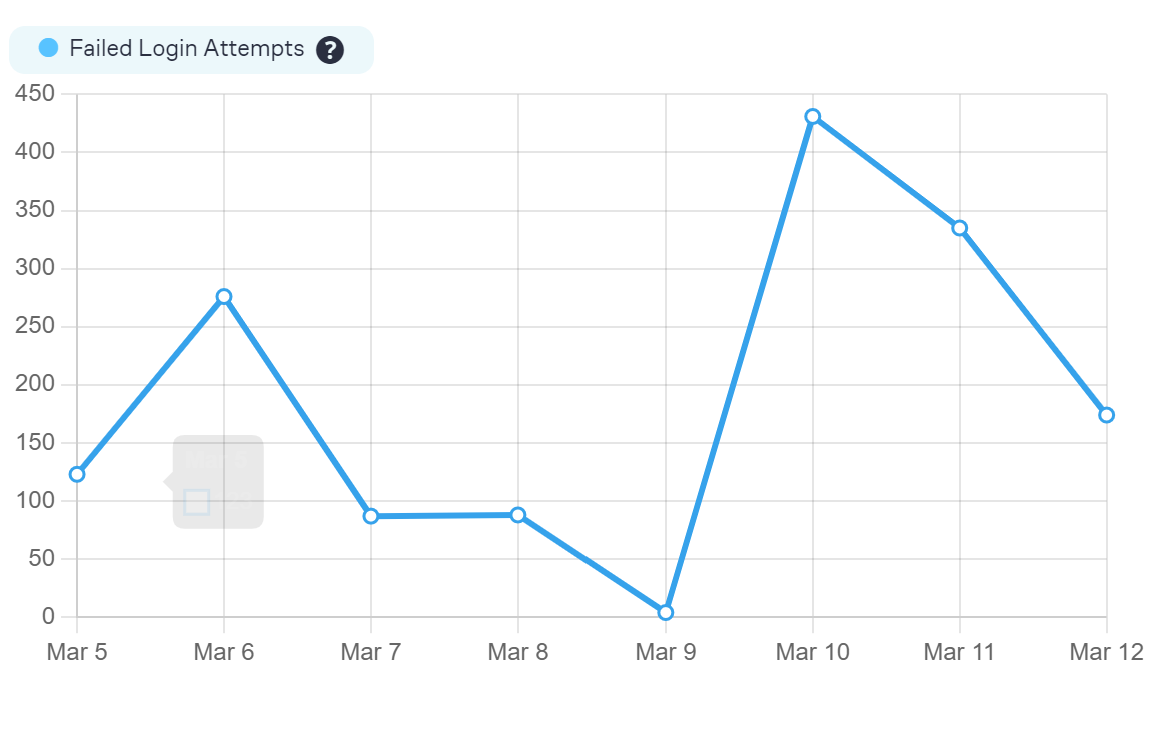
\includegraphics[height=0.3\textheight]{failed_login_attemps_24flow.png}
  \caption[aantal aanvallen op de wordpress website van 24Flow per dag ]{aantal aanvallen op de wordpress website van 24Flow per dag }
\end{figure}
Kleine tot middelgrote IT-servicebedrijven, zoals Sinergio en 24Flow, worden dagelijks geconfronteerd met de uitdaging om hun 
webapplicaties effectief te beschermen tegen cyberaanvallen. Deze bedrijven maken vaak gebruik van populaire webontwikkelingsplatformen 
zoals WordPress en Laravel, die elk unieke en specifieke beveiligingsrisico's en kwetsbaarheden kennen. De bescherming van deze platformen 
wordt vaak toevertrouwd aan de implementatie van beveiligingsplugins en -tools, waarvan de effectiviteit varieert.

Deze bachelorproef richt zich op het onderzoek naar de effectiviteit van verschillende penetratietesttools, zoals Burp Suite, Vega, OWASP ZAP... 
in het identificeren van kwetsbaarheden binnen drie specifieke webomgevingen: een WordPress applicatie zonder beveiligingsplugins,
een WordPress applicatie met beveiligingsplugins en een afgewerkte Laravel applicatie. Het doel van dit onderzoek is tweeledig. 
Ten eerste, het vaststellen welke de meest effectieve penetratietesttool(s) zijn voor deze specifieke webomgevingen. Ten tweede, 
een analyse maken van de beveiligingsrisico's geassocieerd met elk van deze omgevingen om de vraag te beantwoorden hoe onveilig een 
WordPress applicatie zonder beveiligingsplugins werkelijk is. Dit wordt vergeleken met een WordPress applicatie met 
beveiligingsplugins en een Laravel applicatie.

De directe doelgroep voor deze bachelorproef is het bedrijf Sinergio, een kleine IT-serviceprovider die regelmatig 
werkt met WordPress en Laravel voor het ontwikkelen van webapplicaties voor hun klanten. De resultaten van dit 
onderzoek biedt Sinergio waardevolle inzichten in de meest effectieve manieren om hun webontwikkelingsprojecten beter 
te beveiligen. Dit stelt hen bovendien in staat om geïnformeerde beslissingen te nemen over de implementatie van 
beveiligingsstrategieën en -tools. Sinergio zal zo kunnen achterhalen welke pentesting tool het interessantste is binnen hun specifieke omgevingen.
Bovendien draagt dit onderzoek bij aan een bredere kennisbasis over webapplicatiebeveiliging, 
wat van belang kan zijn voor andere kleine tot middelgrote IT-bedrijven die vergelijkbare technologieën gebruiken.

\section{\IfLanguageName{dutch}{Onderzoeksvraag}{Research question}}%
\label{sec:onderzoeksvraag}
Hoe variëren de prestaties van verschillende penetratietesttools bij het identificeren van kwetsbaarheden binnen de drie 
specifieke webomgevingen. Welke specifieke kwetsbaarheden detecteren de penetratietesttools in een WordPress-omgeving zonder 
beveiligingsplugins en hoe verschilt dit van de omgevingen met beveiligingsplugins en de Laravel-applicatie? 
In hoeverre verbeteren beveiligingsplugins de detectiecapaciteiten van deze tools op een WordPress-site? 
Tot slot zal dit onderzoek de beveiligingsniveaus van een onbeveiligde WordPress-website vergelijken met die 
van een beveiligde site en een Laravel-applicatie, om zo te bepalen hoe de aanwezigheid van beveiligingsplugins de 
veiligheid beïnvloedt.

\section{\IfLanguageName{dutch}{Onderzoeksdoelstelling}{Research objective}}%
\label{sec:onderzoeksdoelstelling}
De doelstelling van deze paper is het uitvoeren van een vergelijkende studie. Deze studie evalueert de effectiviteit van 
verschillende penetratietesttools bij het identificeren van kwetsbaarheden in drie specifieke webomgevingen: een WordPress-website 
zonder beveiligingsplugins, een WordPress-website met beveiligingsplugins en een volledig ontwikkelde Laravel-applicatie.
Het beoogde resultaat is een verslag met gedetailleerde aanbevelingen over de meest effectieve tools voor elke geteste 
omgeving. Het succes wordt gemeten aan de hand van de volledigheid van de verzamelde data, de analytische diepgang van de bevindingen, 
en de duidelijkheid van de vergelijkende analyse tussen de tools en omgevingen. Dit verslag zal essentiële inzichten bieden die 
bijdragen aan betere beveiligingsstrategieën en -implementaties in webontwikkelingsprojecten.
\section{\IfLanguageName{dutch}{Opzet van deze bachelorproef}{Structure of this bachelor thesis}}%
\label{sec:opzet-bachelorproef}

% Het is gebruikelijk aan het einde van de inleiding een overzicht te
% geven van de opbouw van de rest van de tekst. Deze sectie bevat al een aanzet
% die je kan aanvullen/aanpassen in functie van je eigen tekst.

Het verdere verloop van deze bachelorproef ziet er uit als volgt:

Hoofdstuk~\ref{ch:stand-van-zaken} geeft een overzicht van de stand van zaken binnen het onderzoeksdomein, op basis van een literatuurstudie.

Hoofdstuk~\ref{ch:methodologie} geeft toelivhting omtrent de methodologie en de gebruikte onderzoekstechnieken die een antwoord te kunnen formuleren op de onderzoeksvragen.

% TODO: Vul hier aan voor je eigen hoofstukken, één of twee zinnen per hoofdstuk
Hoofdstuk~\ref{ch:resultaten}, bevat de resultaten van het onderzoek.

Hoofdstuk~\ref{ch:conclusie}, tenslotte, wordt de conclusie gegeven en een antwoord geformuleerd op de onderzoeksvragen. Daarbij wordt ook een aanzet gegeven voor toekomstig onderzoek binnen dit domein.